\chapter{User interface design}

\section{Mock-ups}
We have already presented the mock-ups for mobile and desktop versions of the app in section 2.2.1 of the Requirements analysis and specification document.

\section{UX diagrams}
In this section UX diagrams for some of the relevant operations will be showed in order to better describe the user interaction with the system.

\begin{figure}[h]
	\centering
	\includegraphics[width=6cm,keepaspectratio]{figures/resv_ux_diagram.eps}
	\caption{UX user with active reservation}
	\label{fig:resv_ux_diagram}
\end{figure}

\begin{figure}[h]
	\centering
	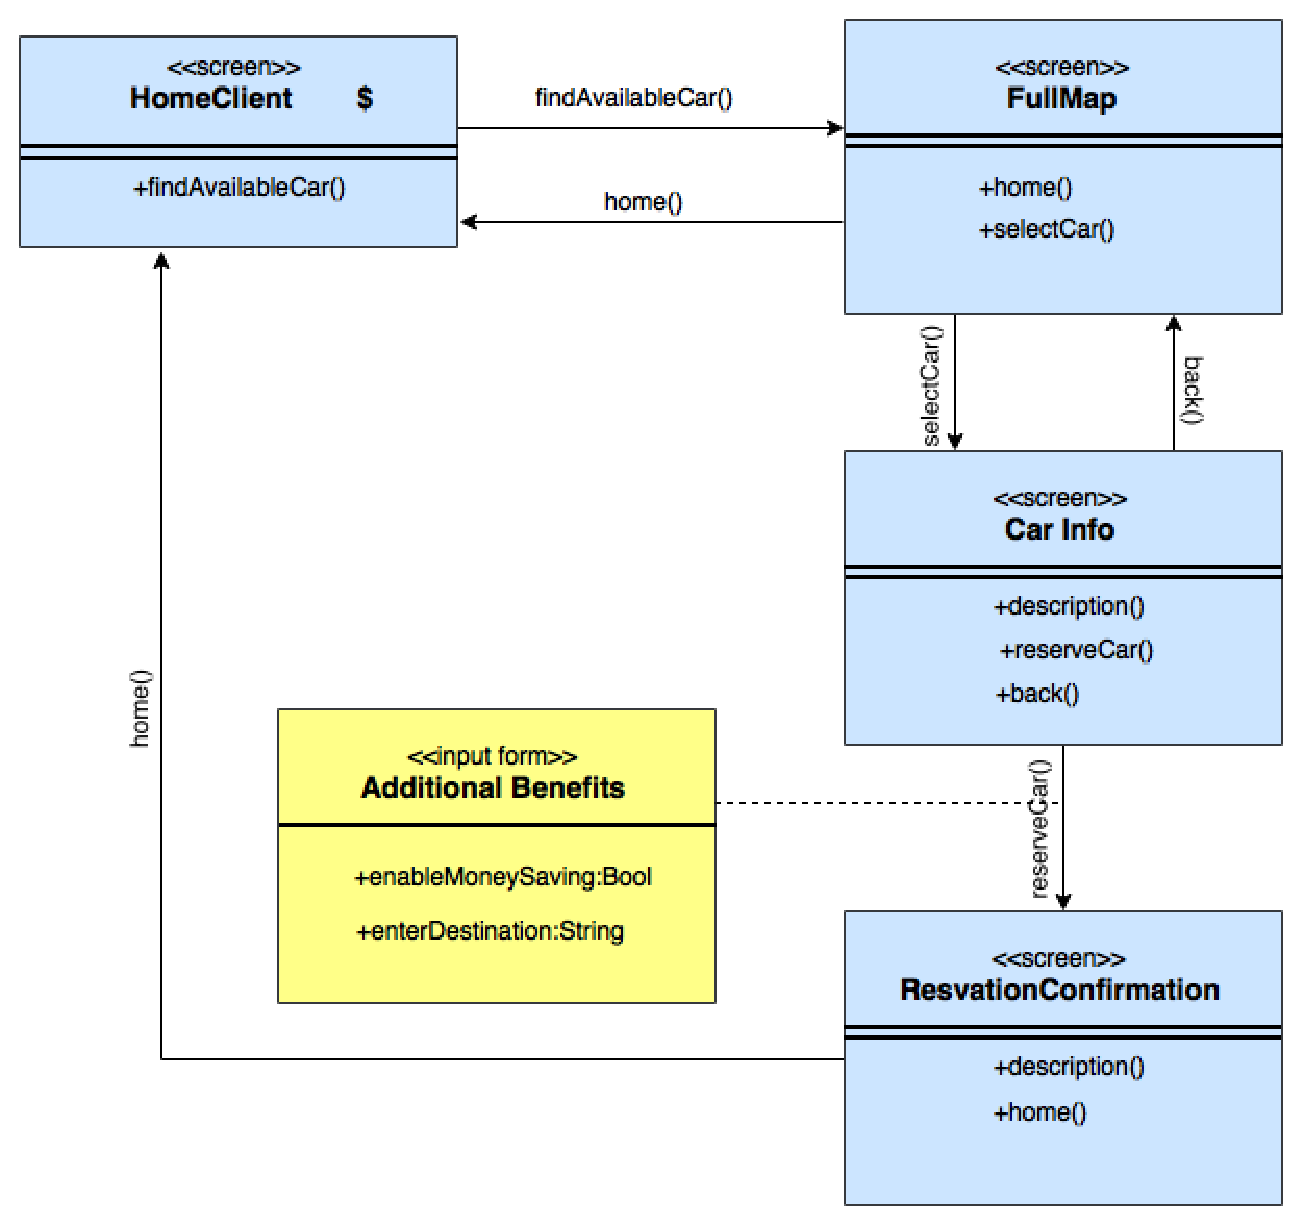
\includegraphics[width=\linewidth,keepaspectratio]{figures/notresv_ux_diagram.eps}
	\caption{UX user with no reservation}
	\label{fig:notresv_ux_diagram}
\end{figure}

\clearpage
\section{BCE diagram}
The figure~\ref{fig:bce_diagram} shows the Business-Controller-Entity diagram for users that access to the homepage not having an active reservation of a car. A BCE diagram is very useful when the MVC pattern is used as arch
\begin{figure}[h]
	\centering
	\includegraphics[height=14cm,keepaspectratio]{figures/bce_diagram.eps}
	\caption{BCE user with no reservation}
	\label{fig:bce_diagram}
\end{figure}